\documentclass[12pt]{article}

\usepackage{fancyhdr}
\usepackage{geometry}
\usepackage[utf8]{inputenc}
\usepackage[T1]{fontenc}
\usepackage[english]{babel}
\usepackage{amsmath,amssymb,amstext}
\usepackage{hyperref}
\usepackage{cancel}
\usepackage{dsfont}
\usepackage{physics}
\usepackage{mathrsfs}
\usepackage{lmodern}
\usepackage{enumerate}
\usepackage{enumitem}
\usepackage{graphicx}
\usepackage{listings, color}
\usepackage[labelfont=bf]{caption}
\usepackage{titling}
\usepackage{siunitx}
\usepackage{tikz}
\usepackage{icomma}
\usepackage{revsymb}
\usepackage{overpic}
\usepackage{subfigure}

\usepackage[backend=biber,backref=false,style=numeric-comp, sorting=none,block=ragged,firstinits=true]{biblatex}

\lstset{basicstyle=\scriptsize,breaklines=true} %Quellcode mit Umlauten und ganz klein
\lstset{literate=
	{Ö}{{\"O}}1
	{Ä}{{\"A}}1
	{Ü}{{\"U}}1
	{ß}{{\ss}}2
	{ü}{{\"u}}1
	{ä}{{\"a}}1
	{ö}{{\"o}}1
}


%Geometrie----------------------------------------------------------------------------------------------------------

\geometry{a4paper, top=25mm, left=15mm, right=15mm, bottom=25mm,headsep=10mm, footskip=10mm}
\pagestyle{fancy}
\setlength{\parindent}{0pt} %Zeileneinrückung

\fancyhf{} %Setzt voreingestellte Kopf-und Fußzeilen-Eigenschaften zurück

\lhead{\nouppercase{\leftmark}}
\chead{}
\rhead{\thepage}

\lfoot{}
\cfoot{}
\rfoot{}

\title{\vspace{0cm}{\Huge Fortgeschrittenen-Praktikum II:\\ \vspace{1cm} Holography}}
\author{Saskia Bondza\\Simon Stephan}
\date{conducted from 27.02.2017 to 10.03.2017}

\pretitle{%
	\begin{center}
		\LARGE
		
\includegraphics[width=6cm,]{../figures/siegel}\\[\bigskipamount]
	}
	\posttitle{\end{center}}

%neue Commands----------------------------------------------------------------------------------------------------------
\newcommand{\nab}{\vec{\nabla}} %direkter Befehl mit Vektorpfeil
\newcommand{\sinc}{\mathrm{sinc}}
\newcommand{\degree}{^\circ}
\newcommand{\gra}[3][0.7]{
	\begin{minipage}[h!]{\textwidth}
		\centering
		\includegraphics[width=#1\textwidth]{../figures/#2.png}
		\captionof{figure}{#3}
	\end{minipage}
	\vskip 30 pt
}
\newcommand{\graX}[4][0.7]{
	\begin{minipage}[h!]{\textwidth}
		\centering
		\includegraphics[width=#1\textwidth]{../figures/#2.png}
		\captionof{figure}[#3]{#4}
	\end{minipage}
	\vskip 30 pt
}
\newcommand{\graTwo}[4][0.49]{
	\begin{minipage}[h!]{\textwidth}
		\centering
		\includegraphics[width=#1\textwidth]{../figures/#2.png}
		\includegraphics[width=#1\textwidth]{../figures/#3.png}
		\captionof{figure}{#4}
	\end{minipage}
	\vskip 30 pt
}
\newcommand{\graXTwo}[5][0.49]{
	\begin{minipage}[h!]{\textwidth}
		\centering
		\includegraphics[width=#1\textwidth]{../figures/#2.png}
		\includegraphics[width=#1\textwidth]{../figures/#3.png}
		\captionof{figure}[#4]{#5}
	\end{minipage}
	\vskip 30 pt
}
\newcommand{\graXTwoB}[6]{
	\begin{minipage}[h!]{\textwidth}
		\centering
		\includegraphics[width=#1\textwidth]{../figures/#3.png}
		\includegraphics[width=#2\textwidth]{../figures/#4.png}
		\captionof{figure}[#5]{#6}
	\end{minipage}
	\vskip 30 pt
}
\newcommand{\graXThree}[6][0.49]{
	\begin{minipage}[h!]{\textwidth}
		\centering
		\includegraphics[width=#1\textwidth]{../figures/#2.png}
		\includegraphics[width=#1\textwidth]{../figures/#3.png}
		\includegraphics[width=#1\textwidth]{../figures/#4.png}
		\captionof{figure}[#5]{#6}
	\end{minipage}
	\vskip 30 pt
}
\newcommand{\graTwoB}[5]{
	\begin{minipage}[h!]{\textwidth}
		\centering
		\includegraphics[width=#1\textwidth]{../figures/#3.png}
		\includegraphics[width=#2\textwidth]{../figures/#4.png}
		\captionof{figure}{#5}
	\end{minipage}
	\vskip 30 pt
}
\newcommand{\del}[2][]{\frac{\partial #1}{\partial #2}}
\newcommand{\code}[1]{\texttt{#1}}

\addbibresource{fp_refs.bib}

%Titel,Inhalt----------------------------------------------------------------------------------------------------------

\begin{document}
	\pagenumbering{gobble} %verstecke Seitenzahl
	\maketitle
	\newpage
	

	
	\section*{Abstract}
	
	\newpage
	
	\thispagestyle{empty}
	\tableofcontents
	\newpage
	
	%Schreiben----------------------------------------------------------------------------------------------------------
	\pagenumbering{arabic}
	
	\section{Introduction and Objective}

Holography is a procedure used to obtain three dimensional images of objects. Unlike photographies that only save information about the intensity of the light and therefore only produce a two dimensional image, holograms also store phase information using an interference based technique. 
Since Denis Gabor developed the theoretical fundament for the holography technique in 1947 and the development of the Laser providing a coherent light source in 1963 and therefore making holography a feasible method, there have been multiple applications making great use of holograms.
A few examples are holograms on paper money to make it more difficult to copy it or the use of holography in archeology to protect finds while still being able to analyze them or, as in case of this experiment, very precise measurements.\\
This experiment is split up into four parts. In a first part the coherence length of a Helium Neon Laser used as light source in all further parts of the experiment is determined using a Michelson Interferometer. In the second part we measure the elastic modulus of three beams made of aluminum, brass and steel using a double exposure holography technique. The objective of the third part of the experiment is to determine the resonant frequencies of an Aluminum plate which is done by using time average holography. In the last part we use Fourier interferometry, a technique based on basic Fourier Optics, to determine the Cross-Correlation of a slit with a slit tilted to the first one. We will use rotations from $0-90\degree$ in $15\degree
$ steps.\\
In order to conduct and understand this experiment a solid background in wave optics, Fourier optics, different Holography techniques as well as understanding of the working of the experimental apparatus is required and will be provided in the following.
	\newpage
	\section{Theoretical Background}

In the following section the theoretical knowledge necessary to understand and perform the experiment will be discussed.

\subsection{Maxwell Equations}

Light is described by electromagnetic waves with a wavelength in a range of $400-800\,\mathrm{nm}$. The behavior and propagation of electromagnetic waves is governed by Maxwell equations which in its source-free form are given as follows:

\begin{align}
	\nab \vec{E}&=0\\
	\nab \vec{B}&=0\\
	\nab\times\vec{E}&=-\del[\vec B]{t}\\
	\nab\times\vec{B}&=\frac1{c^2}\del[\vec B]{t}\text{ ,}
\end{align}
from which we obtain the electromagnetic wave equations:
\begin{align}
	\Delta \vec{E} + \frac{1}{c^2} \ddot{\vec{E}}&= 0\\
	\Delta \vec{B} + \frac{1}{c^2} \ddot{\vec{B}}&= 0\text{ ,}
\end{align}

where the electric field is denoted by E and the magnetic field by B respectively. It can easily be shown that the solutions of these differential equations are given by waves which gives the equations their name.\cite{demtroeder2} In the following we will only consider the electric field when talking about waves for simplicity. Two particular solutions, plane and spherical waves, will be discussed in more detail in the following paragraphs.
\paragraph{Plane Waves}

This solution of Maxwell equations describes a monochromatic, homogeneous plane wave. The amplitude of such a wave will be given by a sinusoidal function of the position r and time t. Practically ideal plane waves aren't possible as they would have to fill all space and be of infinite extent in order to propagate as plane waves. However, plane waves often yield a good approximation locally. Plane waves are described as follows:

\begin{align}
E\left(r, t \right) = E_0 e^{i(kr-\omega t + \phi)}
\end{align}

where k denotes the wave vector and $\omega$ the angular frequency with the dispersion relation $\omega = ck$ and $\phi$ the phase of the wave.
\paragraph{Spherical Waves}

The equation governing monochromatic spherical waves in three dimensions is

\begin{align}
E(r, t) = \frac{E_0}{r}e^{i(kr-\omega t+\phi)}\text{ .}
\end{align}

The equiphase surface for spherical waves is a sphere giving them their name.
\subsection{Interference \label{Interference}}

Interference is a characteristic phenomen for waves and can occur when two (or more) waves ``meet''. The reason for this is that instead of the intensities of the waves being simply add up, the electric fields of the waves are added in accordance to their phase relation. We now want to discuss the interference of two plane waves $E_1(r, t)$ and $E_2(r, t)$ with the time-independent component given by:
\begin{align}
A_1(r) &= E_1 e^{i(k_1r+\phi_1)}\\
A_2(r) &= E_2 e^{i(k_2r+\phi_2)}
\end{align}

where the absolute value of the wave vector k is the same as we are considering waves of the same frequency, the index is indicating different directions of propagation. This leads to the following for the intensity:

\begin{align*}
I(r )&=\left( A_1(r) + A_2(r)\right) \left( A_1(r) + A_2(r)\right) ^*\\
     &= E_1^2 + E_2^2 + E_1E_2e^{i(r(k_1-k_2)+(\phi_1-\phi_2))} +  E_1^2 + E_2^2 + E_1E_2e^{i(r(k_1-k_2)+(\phi_1-\phi_2))}
\end{align*}
Using the relations $2\cos(x) = e^{ix} + e^{-ix}$, $I_i=E_i^2$ as well as $\Delta \delta = r(k_1 - k_2) +(\phi_1-\phi_2)$ this yields:

\begin{align}
I=I_1+I_2 +2 \sqrt{I_1I_2}\cos(\Delta \delta) \label{Intensity}
\end{align}

So the interference pattern of two plane waves will be stripes on a screen as it can be seen in figure \ref{stripies} . \cite{staats}

\graX{stripes}{Interference of two plane waves}{Interference of two plane waves \label{stripies} \footnotemark}
\footnotetext{http://www.mdpi.com/2072-666X/2/2/221/htm}

The interference for a spherical waves and a plane wave can be calculated in the same way. This gives the following result:

\begin{align}
I=I_1+I_2+2\sqrt{I_1I_2}\cos(k(r-x\sin\theta))
\end{align}



\subsection{Coherence \label{Coherence section}}

Coherence is an ideal property of light waves enabling the phenomenon of interference discussed in the previous section. It is in principle defined as the degree of correlation of physical quantities of a single wave or between multiple waves or even wave packets. This degree of correlation can vary between $0$ which is the case for complete incoherence and $1$ which describes waves perfectly coherent. In other words, coherence describes the ability to make predictions of the physical quantities of a wave at one point from knowing what it looks like at another point (see figure ). There are two types of coherence, namely temporal and spatial coherence which are further discussed below. Theoretically, plane waves as well as spherical waves should be perfectly coherent, however this is not the case in reality. Instead there is are physical quantities called the coherence length and time, describing over which spatial and temporal extension a given wave can be seen as coherent. Two sources are described as perfectly coherent if they have the same phase difference and the same wavelength. In principle this is the reason that interference can only be observed for coherent waves. For coherent waves the intensity in a point where two waves with intensities $I_1$ and $I_2$ and phase difference $\Delta \phi$ hit, is given by

\begin{align}
I=\left| a_1 e^{i \phi_1} + a_2 e^{i \phi_2} \right|^2 = \left(I_1+I_2 \right) \left[ 1 + m \cos(\Delta \delta)\right], 
\end{align}

which we have seen in equation \ref{Intensity} when discussing the interference of two plane waves.
While for incoherent waves one only observes the time average as the phase difference is not constant, the phase delay is changing rapidly and the $cos(\theta)$ fluctuations average out to zero. This results in the following over all intensity for two incoherent waves:

\begin{align}
I=\left| a_1 e^{i \phi_1} \right|^2+ \left| a_2 e^{i \phi_2}\right|^2 = I_1+I_2
\end{align}

This makes it obvious that interference is not observable for incoherent light.\cite{coherence}



\graX[]{Coherence}{Spatial and Temporal coherence of wavelets}{Spatial and Temporal coherence of wavelets: \textbf{left} spatial and temporal coherent wave \textbf{middle:} Spatial coherent and temporal incoherent wave \textbf{right:} incoherent wave \label{Coherence} \footnotemark}
\footnotetext{https://i.stack.imgur.com/U9JsT.png}

\subsubsection{Temporal Coherence}
We speak of a wave packet being temporal coherent, if two measurements of a field with a temporal separation $\tau$ fulfill the following condition:

\begin{align}
\Delta \phi \left( t \right) - \phi\left( t + \tau\right)  = \text{const.}
\end{align}

As this is equivalent to two measurements in longitudinal direction, temporal coherence is also referred to as longitudinal coherence. The maximum temporal separation $tau_c$ which still fulfills the previously mentioned condition for a given wave package is defined as the coherence time and is given by:

\begin{align}
\tau_c = \frac{1}{\Delta \nu} \approx\approx \frac{\lambda^2}{c\Delta \lambda}
\end{align}

A straight forward way to measure the coherence time and the longitudinal coherence respectively is the Michelson interferometer which is also used in this experiment and described in section REF.
\subsubsection{Spatial Coherence}
Spatial Coherence, also referred to as Transverse Coherence and is defined as constant phase relation between two points that are shifted perpendicular to the propagation direction. The maximum distance over which the physical quantities of the waves still correlate to a certain degree is defined as coherence length. An ideal plane wave obviously has an infinite coherence length. The most straight forward method to measure transverse coherence is the Young interferometer commonly referred to as Double Slit experiment.

\subsection{Diffraction}

Diffraction, just like interference, is another characteristic wave phenomena.

\subsection{Fourier Optics}

The Fresnel-Kirchhoff Integral Formula describing the diffraction of light for any given obstacle can easily be derived from the Kirchhoff Integral Theorem. The geometry of the obstacle is given by the aperture function $g$. The Fresnel-Kirchhoff Integral formula states that the field distribution of the light passing through any given obstacle is the Fourier transform of its aperture function (see \ref{FKK}). The intensity distribution in the far field (far field condition: $\frac{W^2}{L\lambda} \ll 1$, where W denotes the size of the aperture and L the distance to the screen) can then be calculated as follows:


\begin{align}
I=|U(x_0)|^2=\left| \int\limits_{-\infty}^{\infty} g(x,y)e^{-ikx}dx \right|^2
\end{align}

with 

\begin{align}
  U(x_0) &= \frac{1}{\lambda L} C \mathscr{F}{g(x, y)}    = \frac{1}{\lambda L} C   \int\limits_{-\infty}^{\infty}  g(x,y)e^{-ikx}dx    &  C  \cdot C^* &= 1                         \label{FKK}
\end{align}
This is called Fraunhofer diffraction. We observe that the Intensity distribution is the absolute value of the Fourier transform squared. For a detailed derivation see REF.
In the following we will discuss Fraunhofer diffraction for a single slit.

\subsubsection{Single Slit}

The aperture function of a single slit with the width b $b$ abd length $l$ is given by

\begin{align}
g(x)=\begin{cases}1 &\mbox{ falls }|x|\leq\frac{b}{2}\\0 &\mbox{ sonst }\end{cases}
\end{align}

Its Fourier Transform is described by the $sinc$ function in the following manner:

\begin{align}
\mathscr{F}\left[ g(x) \right] = \left| b\right| \cdot \sinc\left( \frac{k \cdot b}{2}\right)  = 2 \cdot \left| b\right| \cdot \frac{\sinc\left( \frac{k \cdot b}{2}\right)}{k \cdot b}
\end{align}

\graX{Einzelspalt}{Single Slit}{Fourier optics for a single slit \footnotemark \label{Spalt}}
\footnotetext{https://www.chem.purdue.edu/courses/chm621/text/ft/basiset/rect/rectangle.gif}

The intensity distribution of the Fraunhofer diffraction pattern in the far field is then given by the following relation:

\begin{align}
I = \left| \mathscr{F}\left[ g(x) \right]\right| ^2 = \left( \left| b\right| \cdot \sinc\left( \frac{k \cdot \left| b\right| }{2} \right) \right) ^2
\end{align}




\subsubsection{Convolution and Correlation}

\paragraph{Convolution} is a mathematical operation computing a third function out of two functions $f$ and $g$. It is a rather complex operation that can (in a simplified way) be imagined as ``smearing'' function $f$ with $g$. The exact definition is is given below.

\begin{align}
(f*g)(t)=\int\limits_{-\infty}^{\infty} f(\tau)\cdot g(t-\tau) d\tau \label{Convo1}
\end{align}

As it turns out, convolution of two functions corresponds to a Multiplication in Fourier Space which is known as Convolution Theorem (see REF) and makes things a lot more convenient as this is a lot easier to compute.

\begin{align}
\mathscr{F}(f*g)=const. \mathscr{F}(f)\cdot \mathscr{F}(g)
\end{align}
 An example for the Convolution of two Functions and the corresponding multiplication in the Fourier Space is given in figure \ref{Convo}.
 
 \graX[0.5]{Convolution}{Illustration of the Convolution theorem}{Illustration of the Convolution theorem with the example of the double slit \label{Convo} \footnotemark}\footnotetext{http://www4.uwsp.edu/physastr/kmenning/images/Hecht4.11.F.31.png}

\paragraph{Cross-Correlation} describes the similarity of two functions dependent on the displacement of one relative to another. It is very similar to the mathematical definition of the convolution operation ( see \ref{Convo1}) with the only difference being the plus sign instead of the minus sign in the argument of the $g$ function on the right hand side of the equation:

\begin{align}
(f*g)(t)=\int\limits_{-\infty}^{\infty} f(\tau)\cdot g(t+\tau) d\tau \label{corr}
\end{align}

Comparing \ref{Convo1} and \ref{corr} we see that cross-correlation of two functions $f(t)$ and $g(t)$ corresponds to the convolution of $f^*(-t)$ and $g(t)$. If the two cross-correlated functions happen to be identical, this process is called autocorrelation.
A comparison between Convolution, Cross-Correlation and Autocorrelation is illustrated ib figure \ref{corsscor}. All three are maximized when the two input functions match up. For this reason the autocorrelation function is also referred to as self-similarity function.

\graX[0.5]{correlation}{Visual comparison of convolution, cross-correlation and autocorrelation}{Visual comparison of convolution, cross-correlation and autocorrelation \label{corsscor} \footnotemark} \footnotetext{By Cmglee - Own work, CC BY-SA 3.0, https://commons.wikimedia.org/w/index.php?curid=20206883}

The relations between convolution and cross-correlation can be used in Fourier optics to record the cross-correlation of two objects. In order to achieve this we use a set-up similar to the one displayed in figure \ref{Correlator}. On the left hand side the light wave hit the first slit. Its Fourier transform can be observed in the back focal plane of the first lens. The middle plate is the hologram of the second slit which is positioned in said back focal plane. In the back focal plane (so in the Fourier space so to say) both signals are multiplied and then transformed back by the second lens, so that we observe the convolution of both signals in the back focal plane of the second lens.

\graX[0.7]{Correlator}{4f-Correlator}{4f-Correlator (with no mask in the transform plane) \label{Correlator} \footnotemark} \footnotetext{http://www4.uwsp.edu/physastr/kmenning/images/Hecht4.11.F.26.png}

In the experiment we conducted the set-up is slightly more complex including spatial filters and accordingly two more lenses to expand and ``clean'' the laser beam (see \ref{SF} and \ref{FI}). 
\subsection{Principles of Holography}

In photography only information about the light intensity is stored while all information about the phase is lost resulting in an only two dimensional image. Holography uses a laser beam that is split into an object and a reference beam with a beam splitter and expanded with lenses. 
The reference beam will hit the photo plate directly while the object beam is scatterd/reflected by the object with the scattered/reflected light hitting the photo plate. The interference occuring between object and reference beam retains the phase information while the intensity is stored on the photo plate during the development process creating a sort of complex grid. Illuminating it with the reference wave recreates the first diffraction order of the object beam constructing a three dimensional image of the object.

\begin{minipage}{\textwidth}
	\centering
	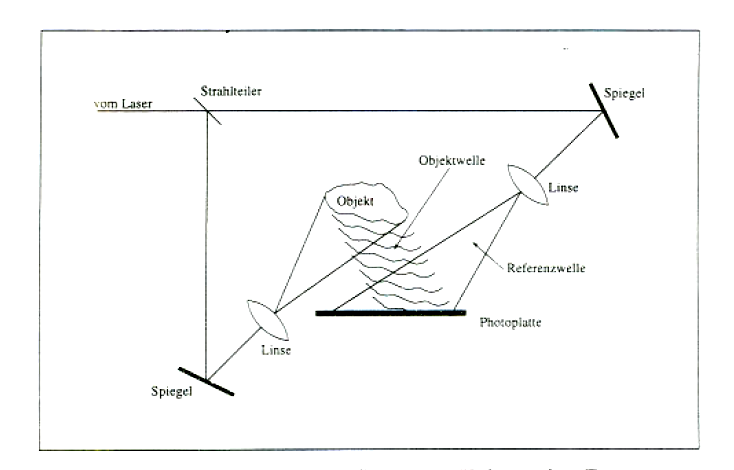
\includegraphics[width=0.5\textwidth]{../figures/holo1}
	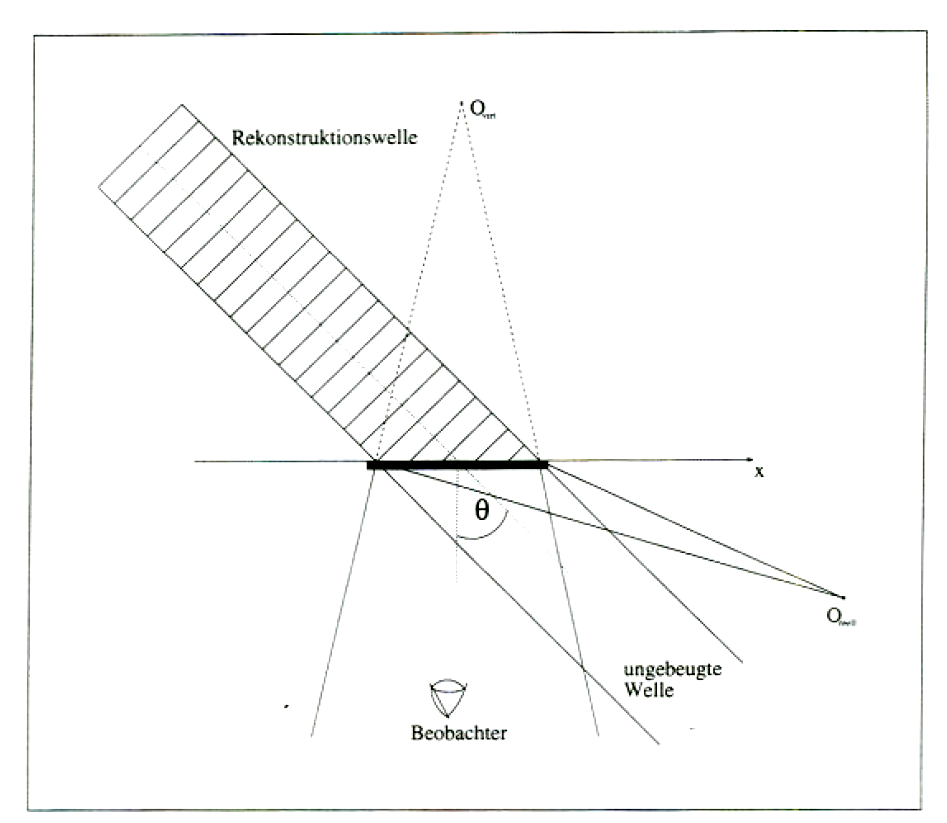
\includegraphics[width=0.4\textwidth]{../figures/holo2}
	\captionof{figure}[Principles of Holography]{left: Set-up to record a Hologram Right: Set up to study a Hologram }
\end{minipage}\vskip 0.5cm



\paragraph{Hologram of a Point}

The holography of a real object can be treated as a ``point cloud'' which means a good understanding of the hologram of a point is fundamental to understand the composition of the hologram of the actual object. 

Let the object wave be a spherical wave that has a certain point $A$ as origin:


\begin{align}
A_1(r)=E_1(r) \ e^{ikr}
\end{align}


The reference wave is a plane wave of the following form:

\begin{align}
A_2(r)=E_2\ e^{ikx \sin\theta} 
\end{align}


The interference of a plane and a spherical wave yields ( as previously discussed in \ref{Interference}):

\begin{align}
I=I_1+I_2+2\sqrt{I_1I_2}\cos(k(r-x\sin\theta))
\end{align}



For $\theta=0\degree$ we obtain an interference pattern made up of multiple circular rings. For  $\theta\neq0\degree$ the interference pattern is distorted, the rings won't be of circular shape.



When the hologram is lit with the reconstruction wave
\begin{align}
A_R(r)=A_R\ e^{ikx \sin\theta},
\end{align}


the time independent component carrying the image information of the electric field is given by:


\begin{align}
A(r)=T_AA_R(r)
\end{align}


where $T_A$ is the amplitude transmission of the photo plate that is calculated by:


\begin{align}
T_A=T_0-Ct_BI
\end{align}


with
$T_0$ and $C$ being constants. $t_B$ denotes the exposure time and $I$ denotes the intensity.
This finally yields the following formula:

\begin{align}
A(r)=\underbrace{[T_0-Ct_B(I_1+I_2)]A_R\ e^{ikx \sin\theta}}_{\mbox{keine Information}} - \underbrace{\sqrt{I_1I_2}A_RCt_B\ e^{ikr}}_{\mbox{vituelles Bild}} - \underbrace{\sqrt{I_1I_2}A_RCt_B\ e^{-ikr}e^{2ikx \sin\theta}}_{\mbox{reelles Bild}}
\end{align}



\begin{itemize}
	\item The first term describes a plane not carrying any relevant information
	\item The second term describes the virtual image as it corresponds to the object wave apart from a varying intensity. When studying the virtual image through the hologram it will be located at the position of the object point $A$.
	\item The third term describes the real image.
\end{itemize}

\subsection{Types of Holograms}

In this section we will discuss the different types of holograms feasible.

\subsubsection{Area and Volume Holograms}

As the photo plate on which the grid for the hologram is formed is not infinitely thin, waves advance into the holography medium interfering in the plate. Thus the grid is not limited to a two dimensional surface, it can be considered three dimensional. As a result, only a certain wavelength hitting the plate in the right angle will reflect to an intensity maximum, similar to Bragg reflexion on a lattice. Seeing that holography only uses laser light of one specific wavelength, the hologram needs to be in the same angle to the reconstruction wave as it was to the reference wave when recording the hologram to reconstruct the object.
We speak of an Area Hologram if the thickness of the plate is of the same order of magnitude as the  wavelength of the light source and of a Volume Hologram if it is much bigger.


\subsubsection{Amplitude- and Phase Holograms}

There are two different types of diffraction gratings: Amplitude gratings and Phase gratings. Amplitude gratings have certain spots allowing light to pass through and others that block it off. As a consequence the amplitude, and thereby the intensity of the light wave, is reduced. Phase gratings on the other hand have different optical densities or different refractive indexes causing phase modulation little effecting the intensity.
The same distinction is feasible for holograms by varying the development technique. In order to achieve an amplitude hologram the silver formed during the development is simply fixed. Bleaching the hologram will turn the silver into a transparent silver halogen effectively transforming the amplitude hologram to a phase hologram. 

\subsubsection{Reflection- and Transmission Holograms \label{ReflTrans}}

During the exposure of the photo plate it is possible to let the object and the reference beam incide from the same side, which we call a transmission hologram, as well as from opposite sides, which we call a reflection hologram. (see figure \ref{RTH1})The alignment of the beams chosen determines from which side one has to study the hologram later to observe the reconstructed image of the object.
As the name suggests a transmission hologram needs to be studied with transmitting light (from the side opposite the inciding reference beam). Likewise a reflection hologram has to be studied in reflected light.

\graX[0.7]{Reflex_Transmissions_Hologram}{Comparison of Reflection and Transmission Hologram}{Comparison of Reflection and Transmission Hologram: a) Recording of a Transmission Hologram b) Recording of a Reflection Hologram c) Studying a Transmission Hologram d) Studying a Reflection Hologram \label{RTH1} \cite{staats}}


\subsection{Holographic Interferometry}

A very precise method to measure small changes in objects and make them visible is the holographic interferometry. The underlying basic principle is to compare the hologram of an object with the hologram of the object in a different state or with the object in a different state itself. Three different types of holographic interferometry, namely Double exposure method, time average method and real time method are described below.

\subsubsection{Double exposure holography}

The double exposure method consists of recording the holograms of the object in two different states on the same photo plate. The exposure time should be the same for both states, so the photo plate is ``double exposed'' giving this method its name. Blocking the object beam and studying the hologram created will then reveal and interference pattern of the two states of the object. This method is used to determine the elastic modulus of various materials in this experiment (see \ref{DEH}).

\subsubsection{Real Time holography}

A hologram of an object at rest is recorded, which is then interfered in ``real time'' with the object making it possible to analyze  and reconstruct movements of an object. This method is highly sensitive to disturbances and it is very important for the set-up to not be moved or changed during the process. 

\subsubsection{Time average holography}

This method has the same underlying principle as real time holography with the difference being that here rather fast processes are observed that the human eye or a camera can't resolve. Effectively, only the spatial component is of significance and observed while the temporal component of the movement is neglected. We use this method to determine resonance frequencies of an aluminum plate (see \ref{RTH}).



\subsection{Elastic Modulus of a Beam \label{EMB}}

A horizontal beam, that is clamped on one side can be considered as multiple layers on top of one another. When this beam deformed by a force acting on it,there will be a middle layer which length stays constant while all other layers will either be stretched or compressed (see figure \ref{beam}).

In the following we will consider a beam of length $a$, width $b$ and depth $c$. We now introduce a reference frame in which the x-axis points in the direction of the length of the beam and a force acts on the beam in negative z-direction.\\

As a result of the deformation two cross sections with the distance $dx$ will be in the angle $d\alpha$ to one another. For the length $l$ of a layer in distance $z$ to the middle neutral layer we therefore obtain the following relation:

\begin{align}
l=(r+z)d\alpha
\end{align}


and for the relative change in length this leads to

\begin{align}
\frac{(r+z)d\alpha-r d\alpha}{dx}=z\frac{d\alpha}{dx}=\frac{z}{r} \label{1}
\end{align}


The elastic modulus of the beam is defined as

\begin{align}
\frac{\Delta l}{l}=\frac{1}{E}\frac{dF}{dzdy} \label{2}
\end{align}


Identifying the previous two relations \ref{1} and \ref{2} with one another yields

\begin{align}
dF=\frac{zE}{r}dzdy
\end{align}

This force cause a momentum compensating the force at the end of the beam ( $x=a$). For small deformations we obtain the differential equation

\begin{align}
\frac{d^2z}{dx^2}=-\frac{12F}{Ebc^3}(a-x)
\end{align}

Double Integration finally leads to the following relation:

\begin{align}
z=-\frac{12F}{Ebc^3}\left(\frac{ax^2}{2}-\frac{x^3}{6} \right)
\end{align}

\graX[0.7]{balken_biegen}{Elastic Modulus of a Beam}{Deformation of a Beam \cite{staats} \label{beam}}

\subsection{Oscillations of an Aluminium Plate \label{Oscillations}}

Aluminum plate with a speaker behind it causing it to oscillate can be considered as driven harmonic oscillator. In the following we want to outline the calculation of the resonant frequencies, exact calculations are too complex to discuss here and can be found in \cite{staats}.
The starting point to derive an equation describing its behavior is the following differential equation:

\begin{align}
\frac{\partial^2 u}{\partial t^2}+\frac{h^2E}{12\rho(1-\mu^2)}\nabla u=0
\end{align}

where $\Delta$ denotes the Laplace-Operator, $h$ denotes the thickness of the plate and $\rho$ its density respectively while $\mu$ is the poisson number of the plate and $E$ its elastic modulus.

Solving this equation yields:

\begin{align}
f_{m\nu}=\frac{x_{m\nu}^2h}{2\pi R^2}\sqrt{\frac{E}{12\rho(1-\mu^2)}} \label{resfreq}
\end{align}

The $x_{m\nu}$ values are the numerical solution to the following equation:

\begin{align}
J_m(ix)\left[ J_{m-1}(x) - J_{m+1}(x)  \right]  - iJ_m(x)\left[ J_{m-1}(ix) - J_{m+1}(ix)  \right] = 0
\end{align}

with $J$ denoting the Bessel functions of the first kind. Solving these equation (which was done using Mathematica) for $x_{m\nu}$ and then subbing this in in \ref{resfreq} gives the following results:

{\centering{}
	\begin{tabular}{c|c|c}
		Mode 		& $x_{m\nu}$ & Calculated Frequency [Hz] 	 \\ \hline\hline
		$m=0,\nu=0$	&$3.19622$   &$5082$						\\ \hline
		$m=1,\nu=0$	& $4.61090$  & $10577$					\\ \hline
		$m=0,\nu=1$	& $6.30644$  & $19787$					\\ \hline
		$m=2,\nu=0$	& $5.90568$  & $17352$					\\ \hline
		$m=2,\nu=1$	& $9.19688$  & $42081$					\\ \hline
		$m=1,\nu=1$	& $7.79927$  & $30263$				     \\ \hline
		$m=3,\nu=0$	& $7.14353$  & $25388$                \\ \hline
     	$m=3,\nu=1$	& $10.53670$ & $55235$
	\end{tabular} }\vskip 0.2cm

where we used the following values in \ref{resfreq}:

\begin{itemize}
	\item $ R = (5.0\pm0.5)\,\mathrm{cm}$
	\item $h=5\,\mathrm{mm}$
	\item $E=70\,\mathrm{GPa}$
	\item $\rho = 2700\,\frac{\mathrm{kg}}{\mathrm{m^3}}$
	\item $\mu = 0.34$ 
\end{itemize}



\subsection{Working principles of the Experimentel apparatus}

\subsubsection{Helium-Neon-Laser \label{HeNe1}}

A cavity with partially transparent mirrors is filled with helium and neon gas with a ratio about 10:1. Applying high voltages can achieve ``pumping'' of Helium atoms (pumping medium) to higher energy levels which can than transfer their energy to Neon Atoms (laser medium) by colliding with them. They get than excited to a higher energy level that has a relatively long life time due to forbidden dipole transitions causing population inversion.
The Helium atoms return to the ground state emitting two photons by stimulated emission. Spontaneous emission is suppressed due to the long life time of the excited state. It is important to generate the first stimulated emissions when turning on the laser though.
The energy level system of a Helium-Neon laser is displayed in figure \ref{HeNe}. A helium-Neon laser typically has a wavelength of $632.8\,\mathrm{nm}$

\graX[0.5]{HeNe}{Energy level system Helium Neon Laser}{Functioning principle of the Helium Neon laser: Energy level system and population inversion for pumping and lasing medium \label{HeNe} \footnotemark}\footnotetext{https://lp.uni-goettingen.de/get/text/1804}


\subsubsection{Spatial Filters \label{SF}}

Spatial Filters are used to filter laser light. Undesired noise and interference or diffraction effects caused by dust or dirt as well as higher frequencies can be eliminated by the beam passing through a lens with a very small focal length followed py a pinhole with a diameter of few micrometers. If the desired output beam is supposed to be a parallel beam which is often the case, a second lens is placed behind the pinhole in the distance of the sum of both focal lengths from the first lens. Without the second lens we obtain a spherical wave. The set-up of a spatial filter is illustrated in figure \ref{SF1}. Spatial Filters can be quite difficult to align in a set-up due to the small focal length of the lens and small diameter of the pinhole (see \ref{DEH}).

\graX[0.5]{SpatialFilter}{Spatial Filter}{Set-Up of a Spatial Filter \label{SF1}}

\subsubsection{Holographic Medium}

\subsubsection{Pockels Cell}

Pockel cells are voltage-controlled wave plates. Their operational principle is the Pockels effect as the name suggests. The Pockels effect describes the change of the refracting properties of an opitical medium induced by an electric field, namely altering or causing birefringence which is the property of a medium to have a refractive index depending on the polarization of light and/or the propagation direction of light. It is often quantified by the maximum difference of refractive indexes inherit to a material. The applications of a Pockels cell are numerous. For example it can create a fast shutter, able to alternate between ``open'' and ``close'' in nanoseconds, by varying the optical rotation between $0\degree$ and $90\degree$. Furthermore it can also be used to pulse a laser by preventing the optical feedback with a polarizing prism preventing optical amplification by directing light of a specific polarization out of the resonator. This results in the gain medium to being pumped in a highly excited state. When it saturates in energy the Pockels cell is switched reinstating optical feedback leading to all energy built up being very quickly released in form of a light pulse of very high intensity. This is known as active Q-switching.
The Pockels cell is crucial for the observation of the resonant frequencies of the aluminium plate in the third part of the experiment where the laser needs to be pulsed with a similar pulse seperation as the time period of the oscillations.





	\newpage
	\section{Experimental Set-up and Procedure}

\subsection{Part 1: Michelson interferometer}\label{sec:michelson}

As we have seen interference is crucial for this experiment (see \ref{Interference} ) and as we have further discussed coherence is an essential condition for that (see \ref{Coherence section}). So in the first part of the experiment we determine the Coherence Length of the light source to make sure that the path difference for object and reference beam won't be bigger than that in all following parts. Furthermore we will test how sensitive the set up is to disturbances.\\
As previously mentioned we will be using a Michelson interferometer for this part (see figure \ref{fig: Michelson}). The light beam emitted from the Helium-Neon Laser encounters a beam splitter resulting in two beams propagating independently from one another. They are then reflected back on the beam splitter with a mirror, with both mirrors adjustable in distance (in a classical Michelson set up it is often just one mirror that is adjustable while the other is placed at a fixed distance from the beam splitter). After passing through the beam splitter they then hit a screen where an interference pattern is observed due to the path difference of both beams. However, the interference pattern will only be observed as long the beams are coherent which offers a straight forward way to measure the Coherence length: During the experiment we will change the path difference by moving the mirrors and thereby determine the Coherence length. Furthermore we will study the influence of disturbances such as noise, movement and a fire lighter.


\graTwo[0.5]{Coherence_length}{aufbau_michelson}{Set-up of Meassuring the Coherence Length with a Michelson interferometer \label{fig: Michelson} }


\subsection{Part 2: Double Exposure Hologram - Elastic Modulus of a Beam \label{DEH}}

The set-up used for this part of the experiment can be seen in figure \ref{DEH!}. The alignment of the spatial filters is the crucial part of the set-up and can take some time. A technique to get the spatial filters aligned is given in \cite{anleitung}.
The ratio of the intensities of reference and object beam could be adjusted by turning the beam splitter disk and should ideally be 10:1 at the position of recording the hologram. This can be verified with a photo diode. However, the photo diode turned out to be highly unreliable so that the ratio was estimated with the eye. A guideline can be that the reflection of the beam should just be bright enough to still be distinguishable from the reference beam on the photo plate which should be placed at Brewster angle with respect to the reference beam to minimize reflection. For glass this angle is $56 \degree$. Both beams should hit the centre of the photo plate.  

\graXTwo[0.5]{Versuchsaufbau_2}{aufbau-2}{Set-up for the double-exposure hologram}{top: Set-up for taking the holograms in part 2 and 3 of the experiment bottom: Set-up for taking the double-exposure hologram \label{DEH!}}

For the Double Exposure hologram three baths with developer, bleacher and water are prepared. Based on experience, we chose the following time intervals for the process of recording the hologram:

\begin{itemize}
	\item Exposure: $2 \times 5\,\mathrm{minutes}$
	\item Development: $3\,\mathrm{minutes}$
	\item Pre-watering: $10\,\mathrm{seconds}$
	\item Watering: $2\,\mathrm{minutes}$
	\item Bleaching: $15\,\mathrm{minutes}$
	\item Pre-watering: $10\,\mathrm{seconds}$
	\item Watering: $10\,\mathrm{minutes}$
	\item Cleaning: $1\,\mathrm{minutes}$
\end{itemize}

Once the process was successful and a hologram could be observed, photographs were taken with a digital camera of the hologram and of the beams with a ruler for scaling from the same perspective to ensure the same scaling for all images.



\subsection{Part 3: Real-time Holography - Oscillations of an Aluminium Plate \label{RTH}}

The set up used for this part of the experiment was nearly identical as in the previous section and can be seen in figure \ref{setup3}. Hoewever, here we use a glass plate in a flooding system as recording medium and the object is a round aluminum plate. 
The glass plates were left in a water bath over night before performing the experiment. The set-up was slightly adjusted as the aluminum plate has a different reflectivity and hence the ratio  between object and reference beam needs to be realigned. In order to record the hologram the times for the different parts of the process were slightly varied:

\begin{itemize}
	\item Soaking:  $10\,\mathrm{minutes}$
	\item Exposure: $5\,\mathrm{minutes}$
	\item Development: $3\,\mathrm{minutes}$
	\item Pre-watering: $10\,\mathrm{seconds}$
	\item Watering: $2\,\mathrm{minutes}$
	\item Bleaching: $45\,\mathrm{minutes}$
	\item Pre-watering: $3 \times 30\,\mathrm{seconds}$
	\item Watering: $1\,\mathrm{minutes}$
\end{itemize}

\graX[0.7]{aufbau3}{Experimental Set-up part 3}{Set-up for taking the real-time hologram }{{Set-up for taking the real-time hologram \label{setup3}}

To observe the hologram, the flooding system was refilled with water. The set-up in this part is extremely sensitve to disturbance so the hologram needs to be recorded and observed with extreme caution. Once a hologram was recorded successfully a speaker was placed behind the aluminum plate which was illuminated with the laser in pulsed mode (which can be achieved with the Pockels Cell) and connected to an oscilloscope to observe and optimize the settings. The necessary wiring can be seen in figure \ref{wiring} as well as an ideal signal. 

It is crucial to choose a relatively short pulse duration to observe the interference patterns. Furthermore the settings can be optimized by fine tuning the frequency as well as varying the delay and volume of the speaker.

\graX[0.4]{aufbauschaltung}{ Wiring for the resonance frequencies}{ Wiring for the resonance frequencies \label{wiring}}
\subsection{Part 4: Fourier Interferometry \label{FI}}

The set up used in this part can be seen in figure \ref{setup4}. In this part of the experiment we make particular use of the fact that the Fourier Transform of an object can be observed in the back focal plane of a length as well as the convolution theorem (see \ref{Convo1}). We altered the previous set-up and placed lenses behind the spatial filters to achieve a parallel beam. The reference beam then hits the glass plate without encountering further optical components while a rotatable slit is placed in the object beam. After passing through the slit, the beam then passes through a lens placed in a distance corresponding to the focal length of both slit and glass plate so that the Fourier Transform is recorded. The intenstiy density of both beams should be adjusted to be about the same. Again, the recording times were adjusted and we used a dry plate this time.:

\begin{itemize}
	\item Exposure: $8\,\mathrm{minutes}$
	\item Development: $3\,\mathrm{minutes}$
	\item Pre-watering: $10\,\mathrm{seconds}$
	\item Watering: $2\,\mathrm{minutes}$
	\item Bleaching: $45\,\mathrm{minutes}$
	\item Pre-watering: $3 \times 30\,\mathrm{seconds}$
	\item Watering: $1\,\mathrm{minutes}$
\end{itemize}

\graTwo[0.6]{Versuchsaufbau_4}{aufbau4}{Experimental set-up for the cross-correlation measurement \label{setup4}}

A fourth lens was then placed in the distance of its focal length behind the plate to observe the hologram. Cross-Correlation was recorded in $15\degree$ rotation steps of the slit with a digital camera. However, the hologram was extremely small and difficult to observe. It is important to have sufficient space behind the recording apparatus to place several lenses to magnify the image further if necessary.
	\newpage
	\section{Evaluation}

\subsection{Michelson Interferometer}

In order to observe interference, the beam had to be expanded a fair bit, so that we observed the pattern on the wall as it was not visible with the eye on a screen on the table. The interference pattern observed can be seen in figure \ref{MichelsonInterference}.

\graX[0.7]{michelson1}{Interference pattern - Michelson Interferometer}{Observed interference pattern with the Michelson interferometer (recorded at a path difference of $36\,\mathrm{cm}$) \label{MichelsonInterference}}

Varying the path difference between $0$ and $36\,\mathrm{cm}$ did not have a noticeable impact on the interference pattern leading to the conclusion of a Coherence Length $C_L \geq 36\,\mathrm{cm}$ which is sufficient for the successive parts of the experiment and was considered in future set-ups. Minor Disturbances like talking or walking shook the interference pattern while it completely disappeared when jumping. This was also kept in mind in the next three parts of the hologram meaning movement, noise and other disturbances were kept to an absolute minimum during the exposure while also proceeding extremely carefully in general. 

\subsection{Determination of the Elastic Modulus of different Materials}

Photographs of the hologram were taken with a digital camera as described in \ref{ReflTrans}. In order to determine the position of the interference maxima and minima a ruler was positioned next to each of the beams for scaling paying attention to taking those photos from the same perspective as the photograph of the hologram itself (see figure \ref{Scaling}).

\graXThree[0.5]{staebe1}{staebe2}{staebe3}{Scaling of the interference pattern on the Beams}{Scaling of the interference pattern on the Beams using a ruler \label{Scaling}}


Figure \ref{ELastic} shows the Interference Pattern we were able to observe resulting from the Double Exposure. We used the program Gwyddion (a multiplatform modular free software for visualization and analysis of data) to analyze the interference pattern.  

\graX[0.7]{staebe4}{Interference Pattern on the Beams}{Interference Pattern on the Beams left: Steel middle: Brass three: Aluminium \label{ELastic}}

In a first step we used the photos in figure \ref{Scaling} to calculate the correct conversion between pixels and millimeters. We then used Gwyddion to extrapolate the intensity profile along a beam as it can be seen in figure \ref{stab2gwid} where we folded with a 5 px Gaussian to reduce noise and make the profile smoother as this makes it a lot easier to determine the local minimas. We then export the data and plot them with R determining the local minima of the smooth profile with a simple for loop (see section \ref{code}).  Here and in the following we will do the evaluation for steel. The evaluation for brass and aluminum is entirely analogous and can be found in the appendix (see section \ref{gwyddion}). Note that the Intensity given by Gwyddion does not have a unit, as this is irrelevant for the determination of the elastic modulus this will however not be further considered.\\

The minima in the interference pattern appear at a phase difference of

\begin{align*}
\Delta \varphi=\frac{\pi}{2}(2n+1)\hspace{0.5cm}\mbox{with }n=0,1,2,...,
\end{align*}

as the intensity of interference pattern is proportional to $\cos^2(\Delta\varphi)$. As a conclusion this means that the beam's position due to the deformation $y$ resulting from the weights at the minimum of order $n$ is given by:

\begin{align*}
y=\frac{\lambda}{4}(2n+1)\hspace{0.5cm}\mbox{with }n=0,1,2,... .
\end{align*}

In a next step we plot the deformation $y$ in dependency of $x$. The wavelength of the Helium-Neon Laser is given in \ref{HeNe1}. From \ref{EMB} we know that the correct function to fit is:

\begin{align*}
y(x)=A\cdot\left(5x^2-\frac{1}{6}x^3\right)+Bx+C .
\end{align*}  

The plot and fit we obtain for steel is given in figure \ref{Fit}.

\graXTwoB{0.45}{0.75}{Stab2gwid}{Stab2R1}{Intensity profile of the Interference pattern}{Intensity profile of the Interference pattern. Top: Adaptation of the Photos in Gwyddion; bottom: Extrapolated profile plotted in R (local minima marked in red)\label{stab2gwid}}

\graX[0.7]{Stab2R2}{Fit for the Elastic Modulus of the Steel Beam}{Fit for the Elastic Modulus of the Steel Beam with the parameters: $A=0.02399\pm0.00016$ $B= 0.210\pm 0.006$ and $C= 0.241 \pm 0.011$ \label{Fit}}

With the width  $b=(1.00\pm0.01)\mathrm{cm}$ and the depth  $c=(0.50\pm0.01)\mathrm{cm}$ of the beam as well as the gravitational accelaration $g=9.81\frac{\mathrm{m}}{\mathrm{s}^2}$ and the mass of the weigths the Elastic Modulus is calculated by: 

\begin{align}
E=\frac{12mg}{Abc^3}
\end{align}

The mass of the weight for the steel beam was chosen higher as suggested in the Staatsexamensarbeit \cite{staats} ($m=50\mathrm{g}$ instead of $m=20\mathrm{g}$) as we expect a higher Elastic Modulus and hence less deformation for this material  which might result in less visible interference minima and less data points for the fit.
The error for the Elastic Modulus $E$ was caluclated with Gaussian error propagation.

\begin{table}[h!]
	\centering
	\begin{tabular}{c|c|c|c}
		Material							& Steel (left)	& Brass (middle)	& Aluminum (right)\\ \hline\hline
		meassured $E$ [GPa]			& $196\pm5$	& 	$104\pm3$		& $68.5\pm1.6$			\\ \hline
	literature value \cite{staats} $E_{lit}$ [GPa]	& 195			& 100				& 72
	\end{tabular}
	\caption{Results for the Elastic Modulus}
\end{table}

\subsection{Eigenoscillation of the aluminium plate}

Unfortunately there were various problems with the set-up in this part especially regarding the bleaching, so that the resonant frequency patterns can not be seen as neatly as expected. However, a hologram was obtained good enough to determine the first six resonant frequencies. The photographs taken with a digital camera as well as the reference pictures are presented in figures \ref{ResFreq1}-\ref{ResFreq6}.

\graXTwoB{0.65}{0.34}{aluminium2_edit}{aluminium2_lit}{Oscillation of the aluminium plate at $(441.5\pm0.5)\,\si{Hz}$}{Oscillation of the aluminium plate at $f_{00,exp}=(441.5\pm0.5)\,\si{Hz}$ (left: edited image; right: theoretical image \label{ResFreq1} ( $f_{00,lit}=448\mathrm{Hz}$) \cite{staats})}
\graXTwoB{0.65}{0.34}{aluminium3_edit}{aluminium3_lit}{Oscillation of the aluminium plate at $(1059.0\pm1.0)\,\si{Hz}$}{Oscillation of the aluminium plate at $f_{10,exp}=(1059.0\pm1.0)\,\si{Hz}$ (left: edited image; right: theoretical image ($f_{10,lit}=983\mathrm{Hz}$) \cite{staats})}
\graXTwoB{0.65}{0.34}{aluminium6_edit}{aluminium6_lit}{Oscillation of the aluminium plate at $(1716.0\pm1.0)\,\si{Hz}$}{Oscillation of the aluminium plate at $f_{20,exp}=(1716.0\pm1.0)\,\si{Hz}$ (left: edited image; right: theoretical image ( $f_{20,lit}=1592\mathrm{Hz}$)\cite{staats})}
\graXTwoB{0.65}{0.34}{aluminium7_edit}{aluminium7_lit}{Oscillation of the aluminium plate at $(2061.0\pm1.0)\,\si{Hz}$}{Oscillation of the aluminium plate at $f_{21,exp}=(2061.0\pm1.0)\,\si{Hz}$ (left: edited image; right: theoretical image ($f_{21,lit}=4090\mathrm{Hz}$)\cite{staats})}
\graXTwoB{0.65}{0.34}{aluminium9_edit}{aluminium9_lit}{Oscillation of the aluminium plate at $(2964\pm5)\,\si{Hz}$}{Oscillation of the aluminium plate at $f_{11,exp}=(2964\pm5)\,\si{Hz}$ (left: edited image; right: theoretical image ( $f_{11,lit}=2854\mathrm{Hz}$) \cite{staats})}
\graXTwoB{0.65}{0.34}{aluminium10_edit}{aluminium10_lit}{Oscillation of the aluminium plate at $(5383\pm5)\,\si{Hz}$}{Oscillation of the aluminium plate at $f_{31}=(5383\pm5)\,\si{Hz}$ (left: edited image; right: theoretical image \label{ResFreq6} \cite{staats})}

The frequencies were associated with the modes by comparing with the images given in the Staatsexamensarbeit which conveyed the impression to be conclusive most of the time.

As the lower frequencies seemed to be a lot more sensitive and more fine tuning was necessary, we estimated these errors to be relatively low. For the higher frequencies it got increasingly more difficult to adjust the frequency. Additionally, the resonance pattern seemingly became less sensitive which resulted in higher estimated errors. 
As the resonant frequencies calculated in \ref{Oscillations} are in a different order of magnitude as the ones we measured a comparison between these two was assessed to not be meaningful. Instead, we compare the measured frequencies with the values given in the Staatsexamensarbeit that are listed as literature values in the captions of figures \ref{ResFreq1}-\ref{ResFreq6} and in the following will be referred to as theoretical values.

We observe that the measured frequencies and the theoretical frequencies are not compatible within three standard deviations. However, this does not imply that we need to dismiss our measurements right away. In order to check for possible systematical errors we plot the measured frequencies against the theoretical frequencies. Furthermore we will also plot the measured values in dependance of the $x_{m\nu}^2$ values calculated in \ref{Oscillations} as the expected relation is known to be linear (see \ref{Oscillations}). Those two plots are presented in figure \ref{LinFitResFreq}.

\graXTwo[]{LinFitResFreq}{LinFitResFreq1}{Linear Fit to check Systematical Errors}{Left: Linear Fit of the relation of measured and theoretical frequencies to check for Systematical Errors Right: Linear Fit of the measured frequencies and $x_{m\nu}$ values to validate the measurements adjusted R-square-value: $ 0.9977 $ \label{LinFitResFreq}}

First of all we notice that one of the points makes the impression to be a clear outlier. As it was hard to attribute the observed interference patterns with the right modes due to the problems described earlier when performing the experiment (i.e. poor bleaching) and a resulting poor quality of the hologram, we might not have matched this frequency with the correct mode and therefore neglect it for the Linear Fits and further discussions.
As we can see the slope of the line is equal to one within two standard deviations while the offset is equal to zero within one standard deviation, so there do not seem to be any significant systematical errors. This also speaks in favour of our measurement as this result makes both values seem a lot more compatible and suggests underestimated statistical errors. Simultaneously we also observe that the Linear dependency of the $x_{m\nu}$ values holds up. 


\subsection{Fourier Spectroscopy}

The pictures in figure \ref{correlation} were recorded representing the cross-correlation of two slits. Note that a setting of $0\degree$ here was chosen to be vertical. As the observed pattern was rather small, it was difficult to take pictures with the digital camera and the observed hologram couldn't be resolved as nicely as it was observed with the eye.


\begin{figure}
	\centering
	\begin{overpic}[width=0.3\textwidth,tics=10]
		{../figures/fourier-0-2-edit.png}
		\put(10,85){\Large\textcolor{white}{$\alpha=0\degree$}}
	\end{overpic}
	\begin{overpic}[width=0.3\textwidth,tics=10]
		{../figures/fourier-15-2-edit.png}
		\put(10,85){\Large\textcolor{white}{$\alpha=15\degree$}}
	\end{overpic}
	\begin{overpic}[width=0.3\textwidth,tics=10]
		{../figures/fourier-30-2-edit.png}
		\put(10,85){\Large\textcolor{white}{$\alpha=30\degree$}}
	\end{overpic}
	
	\vspace{0.2 cm}
	
	\begin{overpic}[width=0.3\textwidth,tics=10]
		{../figures/fourier-45-2-edit.png}
		\put(10,85){\Large\textcolor{white}{$\alpha=45\degree$}}
	\end{overpic}
	\begin{overpic}[width=0.3\textwidth,tics=10]
		{../figures/fourier-60-2-edit.png}
		\put(10,85){\Large\textcolor{white}{$\alpha=60\degree$}}
	\end{overpic}
	\begin{overpic}[width=0.3\textwidth,tics=10]
		{../figures/fourier-75-2-edit.png}
		\put(10,85){\Large\textcolor{white}{$\alpha=75\degree$}}
	\end{overpic}
	
	\vspace{0.2 cm}
	
	\begin{overpic}[width=0.3\textwidth,tics=10]
		{../figures/fourier-90-2-edit.png}
		\put(10,85){\Large\textcolor{white}{$\alpha=90\degree$}}
	\end{overpic}
	\caption{Images of the slit for different angles $\alpha$}
	\label{correlation}
\end{figure}

Once can clearly tell that the process of recording the hologram was successful and auto-correlation for $0\degree$ as well as cross-correlation for the other angles can be observed. The angles represent a rough estimation and are given without an error as this is a qualitative measurement. The expected images are presented in figure \ref{FourierFaltungSimulation}. There is a consensus between the experimental images and the simulated ones as far as we can tell with the poor resolution given.
 
\graX[0.55]{FourierFaltung}{Simulations of the Cross-Correlation and Convolution of a Single Slit}{Simulations of the Cross-Correlation and Convolution of a Single Slit \cite{anleitung} \label{FourierFaltungSimulation}}
	\newpage
	\section{Summary}

\subsection{Michelson Interferometer}

With the help of the Michelson Interferometer the coherence length of the Laser was measured to be $C_L \geq 36\,\mathrm{cm}$ which was determined to be sufficient for the experiment as this was the maximum path difference feasible on the optical bench. Furthermore, the sensitivity of the interference pattern was identified to be relatively high so that subsequent parts of the experiment were to be performed with extreme diligence.

\subsection{Determination of the Elastic Modulus of the Beams}

The results for the Elastic Modulus of the Beams are presented in the following table:

\begin{table}[h!]
	\centering
	\begin{tabular}{c|c|c|c}
		Material							& Steel (left)	& Brass (middle)	& Aluminum (right)\\ \hline\hline
		measured $E$ [GPa]			& $196\pm5$	& 	$104\pm3$		& $68.5\pm1.6$			\\ \hline
	literature value \cite{staats} $E_{lit}$ [GPa]	& 195			& 100				& 72
	\end{tabular}
	\caption{Results for the Elastic Modulus}
\end{table}

As we can see the measurement of the Elastic Modulus of Steel seems to have been the most exact and corresponds to the literature value within one standard deviation.  The result for brass is still compatible with the literature value as the discrepancy is no bigger than two standard deviations while the value for Aluminum seems to be off by three standard deviations. This can have a number of reasons.

First off, we used a weight with a higher mass to measure the Elastic modulus for steel as we anticipated a higher Elastic modulus for this material. We were able to observe a higher number of minima as for the other two materials, quite possibly as consequence of this. Hence, there was more data available to fit and extrapolate the value from leading to a quite accurate result.

Simultaneously the different reflectivities of the material led to overexposure in the case of Aluminum making the evaluation and determination of the minima more critical. As the errors are derived from the errors on the fit parameters this is not necessarily considered in the specification of the standard deviation. In general, the errors derived from the fit can be questioned regarding their meaningfulness.

Additionally the scaling of the photographs with Gwyddion could only be adjusted to match reality to a certain degree, as an exact method to rescale the images was not available. This would result in a systematic error regarding the position of the minima. As different photographs were used for different materials, varying systematic errors could have been caused.

\subsection{Eigenoscillation of the aluminium plate}

\subsection{Fourier Spectroscopy}
In the Fourier part we managed to get some pictures of the cross-correlation of the two slots. The pictures seem to be consistent with the theoretically expected pictures but since the seen images were very small it's difficult to compare the pictures with the theoretical ones. Additionally it was very difficult to shoot good pictures of the correlation images because the images were very dark caused by the non-complete bleaching and the difficulty to correctly set the camera's focus. Anyway the cross-correlation was much better to see with bare eyes so we could confirm the consistency of our experiment with the theory.
	\newpage
	\section{Appendix}

\subsection{Anhang}

\begin{minipage}{\textwidth}
	\centering
	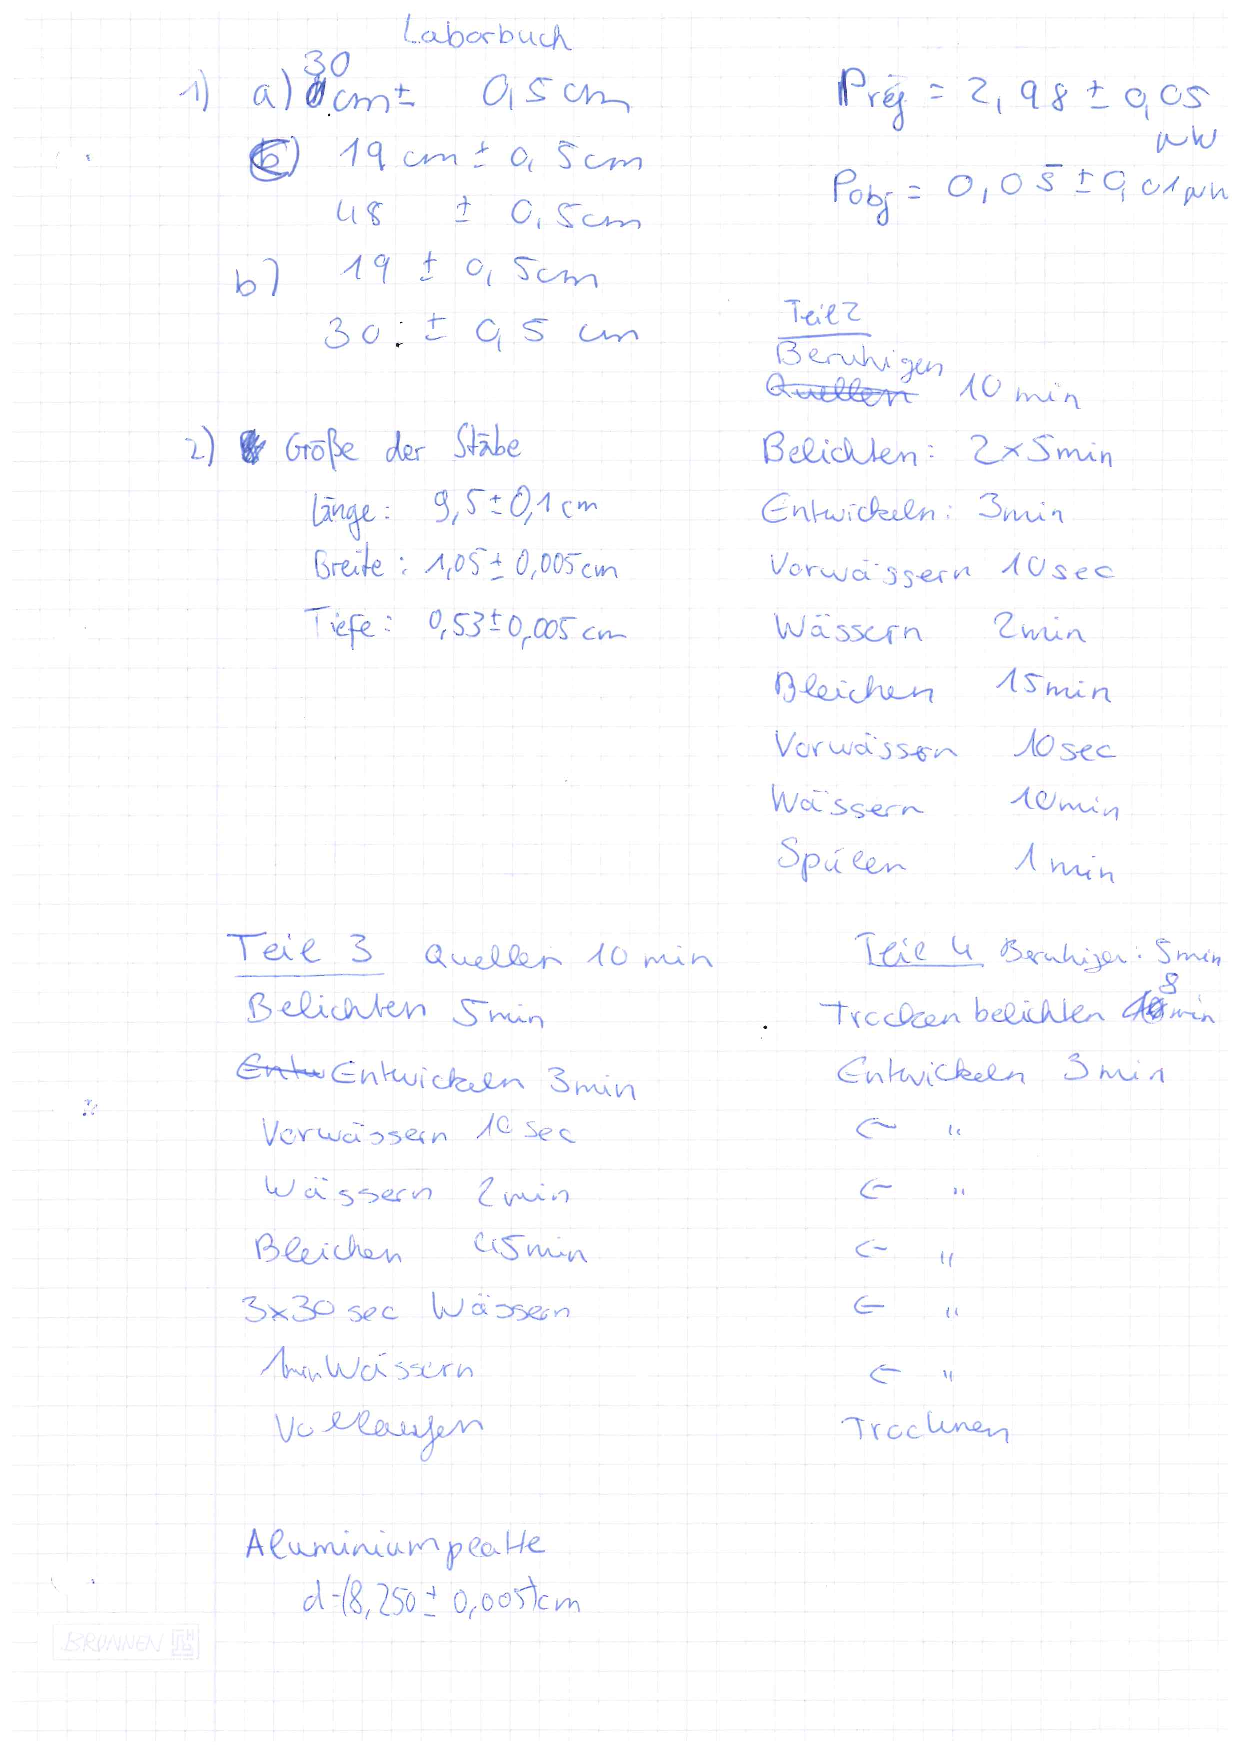
\includegraphics[width=0.9\textwidth]{../figures/Laborbuch1Holo.pdf}
\end{minipage}

\begin{minipage}{\textwidth}
	\centering
	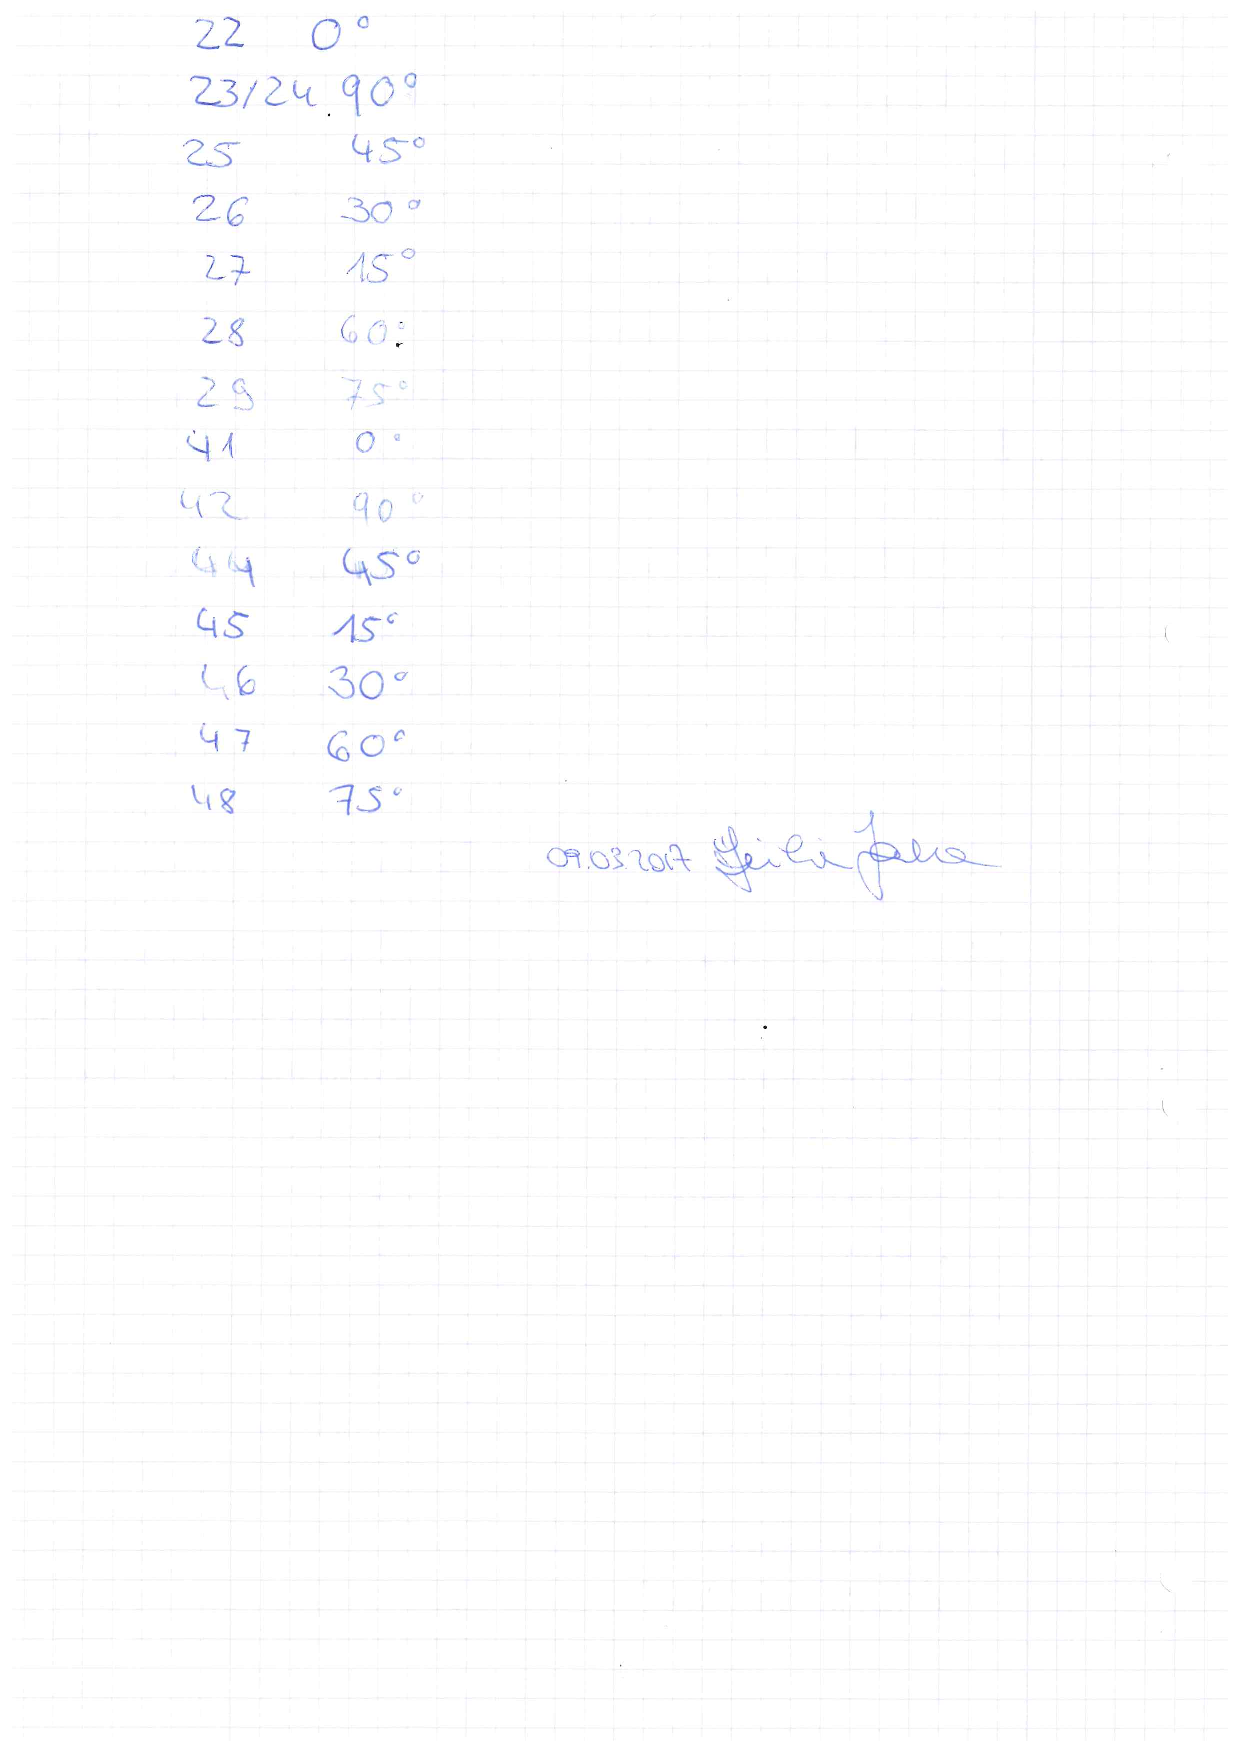
\includegraphics[width=0.9\textwidth]{../figures/Laborbuch2Holo.pdf}
\end{minipage}
	\newpage
	\listoffigures
	\newpage
	\listoftables
	
	%Literatur----------------------------------------------------------------------------------------------------------
	
	%\cite{les}
	\newpage
	\printbibliography[heading=bibintoc]
	
%	\begin{thebibliography}{9}
%		
%		%\bibitem{staat}
%		%  Tobijas Kotyk,
%		%  \emph{Versuche zur Radioaktivität im Physikalischen Fortgeschrittenen Praktikum an der Albert-Ludwigs-Universität Freiburg},
%		%  Albert-Ludwigs-Universität, Freiburg,
%		%  2005
%		
%		
%		
%		%\bibitem{molmasse}
%		%  \emph{http://www.convertunits.com/molarmass/<ELEMENTNAME AUF ENGLISCH>}, Stand 28.09.2015
%		
%		
%		\bibitem{anleitung}
%		M. Köhli,
%		\emph{Versuchsanleitung Fortgeschrittenen Praktikum: SQUID},
%		Albert-Ludwigs-Universität Freiburg,
%		2011
%		
%		\bibitem{staat}
%		Volker Bange,
%		\emph{Einrichtung des Versuches "SQUID"},
%		Albert-Ludwigs-Universität Freiburg,
%		2000
%		
%		\bibitem{chemistry}
%		Bruce A. Averill, Patricia Eldredge,
%		\emph{General Chemistry: Principles, Patterns, and Applications},
%		Saylor Foundation,
%		2011
%		
%		\bibitem{SQUID}
%		Clarke, J.,
%		\emph{SQUIDS},
%		Spektrum der Wissenschaft , 10/1994,
%		Spektrum Akademischer Verlag
%	\end{thebibliography}
	
\end{document}